%                                                                 aa.dem
% AA vers. 8.2, LaTeX class for Astronomy & Astrophysics
% demonstration file
%                                                       (c) EDP Sciences
%-----------------------------------------------------------------------
%
%\documentclass[referee]{aa} % for a referee version
%\documentclass[onecolumn]{aa} % for a paper on 1 column  
%\documentclass[longauth]{aa} % for the long lists of affiliations 
%\documentclass[rnote]{aa} % for the research notes
%\documentclass[letter]{aa} % for the letters 
%\documentclass[bibyear]{aa} % if the references are not structured 
% according to the author-year natbib style

%
\documentclass{aa}  

%
\usepackage{graphicx}
%%%%%%%%%%%%%%%%%%%%%%%%%%%%%%%%%%%%%%%%
\usepackage{txfonts}
%%%%%%%%%%%%%%%%%%%%%%%%%%%%%%%%%%%%%%%%
\usepackage{hyperref}
% To add links in your PDF file, use the package "hyperref"
% with options according to your LaTeX or PDFLaTeX drivers.
%
%\usepackage{url}
%\usepackage{fontawesome}

%\usepackage{xspace}
%\usepackage{subcaption}

\def\detJ{\mathrm{det}J}

\def\reff{R_{\mathrm{e}}}
\def\mstar{M_*}
\def\asps{\alpha_{\mathrm{sps}}}

\def\mobs{M_*^{(\mathrm{obs})}}
\def\gammadm{\gamma_{\mathrm{DM}}}
\def\fdm{f_{\mathrm{DM}}}
\def\mdmfive{M_{\mathrm{DM}, 5}}

\def\tein{\theta_{\mathrm{Ein}}}
\def\teff{\theta_{\mathrm{e}}}
\def\trad{\theta_{\mathrm{rad}}}
\def\tsis{\theta_{\mathrm{Ein}}^{\mathrm{(SIS)}}}
\def\meantsis{<\tsis>}
\def\stdtsis{\sigma(\tsis)}

\def\teinein{\theta_{\mathrm{Ein}}^*}
\def\betaein{\beta^*}

\def\toneobs{\theta_1^{\mathrm{obs}}}
\def\ttwoobs{\theta_2^{\mathrm{obs}}}

\def\moneobs{m_1^{\mathrm{obs}}}
\def\mtwoobs{m_2^{\mathrm{obs}}}

\def\asymm{\xi_{\mathrm{asymm}}}
\def\rmur{r_{\mu_r}}
\def\rmurobs{r_{\mu_r}^{(\mathrm{obs})}}
\def\mumin{\mu_{\mathrm{min}}}
\def\betamax{\beta_{\mathrm{max}}}
\def\betasl{\beta_{\mathrm{SL}}}

\def\hyperpars{\boldsymbol{\eta}}
\def\indpar{\boldsymbol{\psi}}
\def\indpari{\boldsymbol{\psi}_i}

\def\nsource{N_{\mathrm{s}}}
\def\nbkg{n_{\mathrm{bkg}}}

\def\psilens{\boldsymbol{\psi}_\mathrm{g}}
\def\psisource{\boldsymbol{\psi}_\mathrm{s}}
\def\psisourcetwo{\boldsymbol{\psi}_{\mathrm{s},2}}
\def\psisourcens{\boldsymbol{\psi}_{\mathrm{s},\nsource}}
\def\psisourcenobeta{\boldsymbol{\psi}_\mathrm{s}^{(-\boldsymbol\beta)}}

\def\Nlens{N_{\mathrm{lens}}}
\def\Nnot{N_{\mathrm{not}}}

\def\prlens{{\rm P}_\mathrm{g}}
\def\prsource{{\rm P}_\mathrm{s}}
\def\prlensone{{\rm P}_{\mathrm{g},1}}
\def\prlenstwo{{\rm P}_{\mathrm{g},2}}
\def\prsourceone{{\rm P}_{\mathrm{s},1}}
\def\prsourcetwo{{\rm P}_{\mathrm{s},2}}
\def\prsl{{\rm P}_\mathrm{{SL}}}
\def\prslone{{\rm P}_{\mathrm{SL},1}}
\def\prsltwo{{\rm P}_{\mathrm{SL},2}}

\def\prsourcenobeta{{\rm P}_\mathrm{s}^{(-\boldsymbol\beta)}}

\def\pdet{{\rm P}_\mathrm{det}}
\def\pdetone{{\rm P}_{\mathrm{det},1}}
\def\pdettwo{{\rm P}_{\mathrm{det},2}}
\def\crosssect{\sigma_\mathrm{{SL}}}
\def\crosssectps{\sigma_\mathrm{{SL,PS}}}

\def\data{\mathbf{d}}
\def\datai{\mathbf{d}_i}

\def\dlens{\mathbf{d}_{\mathrm{g}}}
\def\dsource{\mathbf{d}_{\mathrm{s}}}

\def\mlim{m_{\mathrm{max}}}

\def\Sref#1{Section~\ref{#1}\xspace}
\def\Fref#1{Figure~\ref{#1}\xspace}
\def\Tref#1{Table~\ref{#1}\xspace}
\def\Eref#1{Equation~\ref{#1}\xspace}

\newcommand{\ale}[1]{\textcolor{red}{\textbf{[Ale: #1]}}}

\def\pr{{\rm P}}

\defcitealias{S+C21}{Paper~I}
\defcitealias{Son21}{Paper~II}
\defcitealias{Son22}{Paper~III}
\setcitestyle{notesep={}}

\begin{document} 


   \title{Strong lensing selection effects}
   \titlerunning{Strong lensing selection effects}
   \authorrunning{Sonnenfeld et al.}

   \author{Alessandro Sonnenfeld\inst{1}
          }

   \institute{Leiden Observatory, Leiden University, Niels Bohrweg 2, 2333 CA Leiden, the Netherlands\\
              \email{sonnenfeld@strw.leidenuniv.nl}
             }

   \date{}

% \abstract{}{}{}{}{} 
% 5 {} token are mandatory
 
  \abstract
  % context heading (optional)
  % {} leave it empty if necessary  
    {
There are selection effects. They are important.
}
  % aims heading (mandatory)
   {
How important?
} 
   % methods heading (mandatory)
   {
We simulate lenses.
}
% results heading (mandatory)
   {
Results.
}
  % conclusions heading (optional), leave it empty if necessary 
   {
We conclude.
}
   \keywords{
             Gravitational lensing: strong 
               }

   \maketitle
%
%________________________________________________________________

\section{Introduction}\label{sect:intro}

Strong gravitational lensing is a powerful tool for studying galaxies and cosmology.
Strong lenses have been used to probe the mass structure of massive galaxies \citep{Aug++10, ORF14, Son++15, Sha++21}, to detect substructure \citep{Veg++12, Hez++16, Nie++20}, to carry out detailed studies of magnified star-forming galaxies \citep{Jon++13}, and to measure the expansion rate of the universe with time delays \citep[see][for a review]{T+M16}.

Strong lenses, however, are a biased subset of the general population of galaxies and background sources.
A necessary condition for a galaxy to act as a strong lens with respect to a given source is that its projected surface mass density $\Sigma(\boldsymbol\theta)$ must be larger than the critical surface mass density for lensing $\Sigma_{\mathrm{cr}}$ at at least one position $\boldsymbol\theta$ \citep{SEF92}.
This condition excludes objects with a very diffuse mass distribution from the population of lenses.
In general, galaxies with a higher concentration of mass are more likely to be strong lenses, and are therefore over-represented in lens samples.

The luminosity and size distribution of strongly lensed sources is also biased with respect to the general population of background galaxies.
For instance, lensing magnification allows the detection of fainter objects with respect to the field, and galaxies that are very extended with respect to the Einstein radius are less likely to be classified as strongly lensed, since their magnification averaged over their size tends to be low \citep[see also the discussion in section 5.3 of][]{O+A17}.

In general, the probability distribution $\prsl$ of a sample of strong lenses from a given survey with selection criterion $S$ is given by \citep{Son22}:
\begin{equation}\label{eq:one}
\prsl(\psilens,\psisource|S) \propto \prlens(\psilens)\prsource(\psisource)\pdet(\psilens,\psisource|S).
\end{equation}
In the equation above, $\psilens$ is the set of parameters describing the properties of foreground galaxies that are relevant for lensing, such as their redshift and mass distribution; $\psisource$ is the set of parameters describing background sources; $\prlens$ and $\prsource$ describe the general distribution of foreground galaxies and background sources in the absence of lensing; and $\pdet$ describes the probability of detecting a lens-source system with parameters $\psilens$ and $\psisource$ given the criterion $S$ used to define a lens.
This last factor takes into account both physical effects, that is whether a lens with parameters $\psilens$ produces a strongly lensed image of a source with parameters $\psisource$, and survey selection effects, that is whether such an image can be recognised as a strong lens.

The left-hand side of \Eref{eq:one} is directly accessible from strong lensing observations. If the main goal of a lensing survey is to characterise the properties of the strong lens population, then it can be accomplished by directly analysing this term. For many applications of strong lensing, however, the aim is to constrain the properties of the general galaxy or source population, $\prlens$ and $\prsource$, which are coupled in a nontrivial way via the lens detection probability $\pdet$.
In order to obtain an unbiased estimate of either $\prlens$ or $\prsource$, then, it is necessary to invert \Eref{eq:one}.
In principle, this can be done with a Bayesian hierarchical formalism, provided that the lens detection probability $\pdet$ is known \citep{Son22}.
For most of the existing strong lensing surveys, however, characterising $\pdet$ is very challenging: the process determining whether a system is included in a strong lens sample is typically a combination of several cuts, usually involving a nontrivial visual selection step. 

The problem of inverting \Eref{eq:one} is a difficult one to tackle exactly.
Few studies have attempted to explicitly account for strong lensing selection effects, usually by making ad-hoc simplifying assumptions \citep{Son++15,O+A17,Son++19}.
%The problem of the invertibility of \Eref{eq:one} can be simplified by adopting lens selection criteria that can be easily forward-modelled: for instance by building samples that are complete above a well-defined observational cut \citep{Son22}.
%The problem can be simplified by adopting lens selection criteria that can be easily forward-modelled: for instance by building samples that are complete above a well-defined observational cut \citep{Son22}.
Whether it is necessary to invert \Eref{eq:one}, however, depends on the severity of the strong lensing bias that needs to be corrected and on the accuracy requirements on the key quantities of interest.

In this paper we aim to quantify the strength of the strong lensing bias on a series of foreground galaxy and background source parameters. %, under realistic assumptions for the lens detection probability $\pdet$.
In particular, we aim to determine how strong lenses differ from the general population of foreground galaxies and background sources in terms of a) the radial mass structure of the lenses (i.e. their stellar and dark matter mass density profiles); b) the ellipticity of the lenses; c) the size-magnitude distribution of the lensed sources.
The answer to this question depends on 1) how the lens detection probability $\pdet$ varies as a function of galaxy and source properties, and on 2) the shape of the galaxy and source parameters distribution $\prlens$ and $\prsource$. To understand this second point we can imagine the limiting case in which both $\prlens$ and $\prsource$ are Dirac delta functions: in this limit, $\prsl$ simply reduces to the product $\prlens\prsource$ up to a scaling constant, corresponding to a case in which the lensing bias is none.

\citet{MVK09} carried out a thorough study of point 1): they quantified how the properties of a lens galaxy determine its probability of creating a lensing event with a point source.
In this work we revisit the \citet{MVK09} study, we expand it to the extended source case and, most importantly, we address point 2) as well: we simulate large populations of strong lenses using empirical models, simulate lensing surveys with realistic assumptions for the lens probability $\pdet$ and quantify the lensing bias under various scenarios.
We explore how the results change as a function of the scatter in mass parameters at fixed light, and as a function of source type: we simulate both galaxy and quasar sources.

%In light of the results of our experiments, we discuss to what extent can studies of galaxy structure based on strong lenses be generalised to describe non-lens galaxies.
Finally, we address the question of how different are galaxy-galaxy lens samples from sets of galaxy-quasar lenses. This last point is relevant for time-delay cosmography studies, in which measurements of the time-delay between the multiple images of a strongly lensed quasar are used to constrain the expansion rate of the Universe. Galaxy-galaxy lenses can in principle be used to help break some of the model degeneracies affecting these measurements \citep{B+T21}, but any difference between the two lens classes can in principle introduce biases, if not corrected for.
With this study we aim to quantify this bias.

The structure of this work is the following.
In \Sref{sect:basics} we introduce the basics of gravitational lensing.
In \Sref{sect:indlenses} we study individual lens systems, to look for trends in the lensing cross-section with various lens and source properties.
In \Sref{sect:lenspop} we describe our simulations of lens populations.
In \Sref{sect:results} we show the results of our analysis on the simulated lens populations.
We discuss the results in \Sref{sect:discuss} and draw conclusions in \Sref{sect:concl}.

The Python code used for the simulation and analysis of the lens sample can be found in a dedicated section of a GitHub repository\footnote{\url{https://github.com/astrosonnen/strong_lensing_tools}}.

%__________________________________________________________________

\section{Strong lensing basics}\label{sect:basics}

The lensing properties of an object with respect to a source depend solely on its dimensionless surface mass density distribution $\kappa(\boldsymbol\theta)$ (also referred to as the convergence). 
This is the ratio between the surface mass density and the critical surface mass density for lensing:
\begin{equation}
\kappa(\boldsymbol\theta) = \dfrac{\Sigma(\boldsymbol\theta)}{\Sigma_{\mathrm{cs}}}.
\end{equation}
%which is the ratio between the projected surface mass density of the lens and the critical surface mass density for lensing.
The latter quantity is defined as
%The quantity $\Sigma_{\matrhrm{cs}}$ is the critical surface mass density for lensing, defined as
\begin{equation}
\Sigma_{cr} = \dfrac{c^2D_s}{4\pi G D_d D_{ds}},
\end{equation}
where $c$ is the speed of light, $G$ the gravitational constant, and $D_d$, $D_s$, and $D_{ds}$ are the angular diameter distances between the observer and the lens, the observer and the source, and the lens and the source, respectively.

Given a source at angular position $\boldsymbol\beta$, images of it form at the positions $\boldsymbol\theta$ that are solutions of the lens equation
\begin{equation}\label{eq:lenseq}
\boldsymbol\beta = \boldsymbol\theta - \boldsymbol\alpha(\boldsymbol\theta),
\end{equation}
where $\boldsymbol\alpha$ is the deflection angle of the lens.
This can be expressed in terms of the dimensionless surface mass density by means of the following integral over the whole sky:
\begin{equation}
\boldsymbol\alpha(\boldsymbol\theta) = \frac{1}{\pi}\int_{\mathbb{R}^2} d^2\boldsymbol\theta' \kappa(\boldsymbol\theta')\dfrac{\boldsymbol\theta - \boldsymbol\theta'}{|\boldsymbol\theta - \boldsymbol\theta'|^2}.
\end{equation}
The images of the background source are in general magnified in total flux and in size, while preserving the original surface brightness.

\subsection{The axisymmetric lens}\label{ssec:axisymm}

In the special case of an axisymmetric lens we can simplify the notation by considering a single coordinate axis with origin at the centre of the lens. We label the components of the image position, source position and deflection angle along this axis as $\theta$, $\beta$ and $\alpha$, respectively.
The lens equation for an axisymmetric lens then becomes
\begin{equation}\label{eq:1dlenseq}
\beta = \theta - \alpha(\theta),
\end{equation}
and the expression for the deflection angle reduces to
%In the special case of an axisymmetric lens, the deflection angle, calculated along an arbitrary axis passing through the lens centre, reduces to
\begin{equation}
\alpha(\theta) = \frac{2}{\theta}\int_0^{\theta} d\theta' \kappa(\theta') \theta'.
\end{equation}
This can also be expressed in terms of the total projected mass enclosed within a circle with angular radius equal to $\theta$:
\begin{equation}
\alpha(\theta) = \frac{1}{\pi\theta}\dfrac{M(<\theta)}{\Sigma_{\mathrm{cr}}D_{\mathrm{d}}^2}.
\end{equation}

A very important quantity for describing the strength of a strong lens is the Einstein radius, $\tein$. For an axisymmetric lens, this is the radius corresponding to the solution of \Eref{eq:lenseq} for a source placed at the same angular position as the lens centre ($\beta=0$).
The circle with radius equal to $\tein$ is known as the tangential critical curve. Images that form here have infinite magnification in the tangential direction.
%
It can be shown that $\tein$ satisfies the following condition,
\begin{equation}\label{eq:criteq}
\bar{\kappa}(<\tein) = 1,
\end{equation}
where $\bar{\kappa}(<\theta)$ is the average surface mass density within a radius equal to $\theta$:
\begin{equation}
\bar{\kappa}(<\theta) \equiv \frac{2}{\theta^2}\int_0^{\theta}d\theta' \kappa(\theta')\theta'.
\end{equation}
%Based on \Eref{eq:criteq},
%we generalise the definition of $\tein$ to the non-axisymmetric case as the circularised radius of the isodensity contour that encloses an average surface mass density equal to $\Sigma_{\mathrm{cr}}$.

Axisymmetric lenses of the kind considered in this work 
%Axisymmetric lenses with a density profile of the kind considered in section \ref{ssec:profile} 
typically produce either one or three images of a point source.
\Fref{fig:scheme} helps to visualise this property.
%\Fref{fig:scheme}, which shows the quantity $\theta - \alpha(\theta)$ as a function of the position in the image plane $\theta$, helps to visualise this property. 
Plotted in \Fref{fig:scheme} is the quantity $\theta - \alpha(\theta)$ as a function of the position in the image plane $\theta$, for a few lens models.
%for the same lens models considered in \Fref{fig:kappa}.
According to \Eref{eq:1dlenseq}, images form at the locations where this quantity equals the position of the source. 
Therefore, given a source position $\beta$, the number of images and their location can be determined by drawing a horizontal line at the value $\beta$ on the vertical axis, and finding the points where this line intersects the $\theta - \alpha(\theta)$ curve.

For small values of $\beta$ (for sources close to the lens centre), the number of images that are produced is three: the source is strongly lensed. For large values of $\beta$, instead, only one image is formed.
The value of $\beta$ where the transition occurs is known as the radial caustic, which is marked by the horizontal dotted line in \Fref{fig:scheme}. 
As can be seen from \Fref{fig:scheme}, a source at this location is mapped to the stationary point of the $\theta - \alpha(\theta)$ curve. 
%this value corresponds to the stationary point of the $\theta - \alpha(\theta)$ curve. 
That location on the image plane is known as the radial critical curve. 
Images that form there have a formally infinite magnification in the radial direction\footnote{The slope of the $\theta - \alpha(\theta)$ curve is the inverse of the radial magnification. This can be understood by taking the derivative of \Eref{eq:1dlenseq} with respect to $\theta$.}.

\begin{figure}
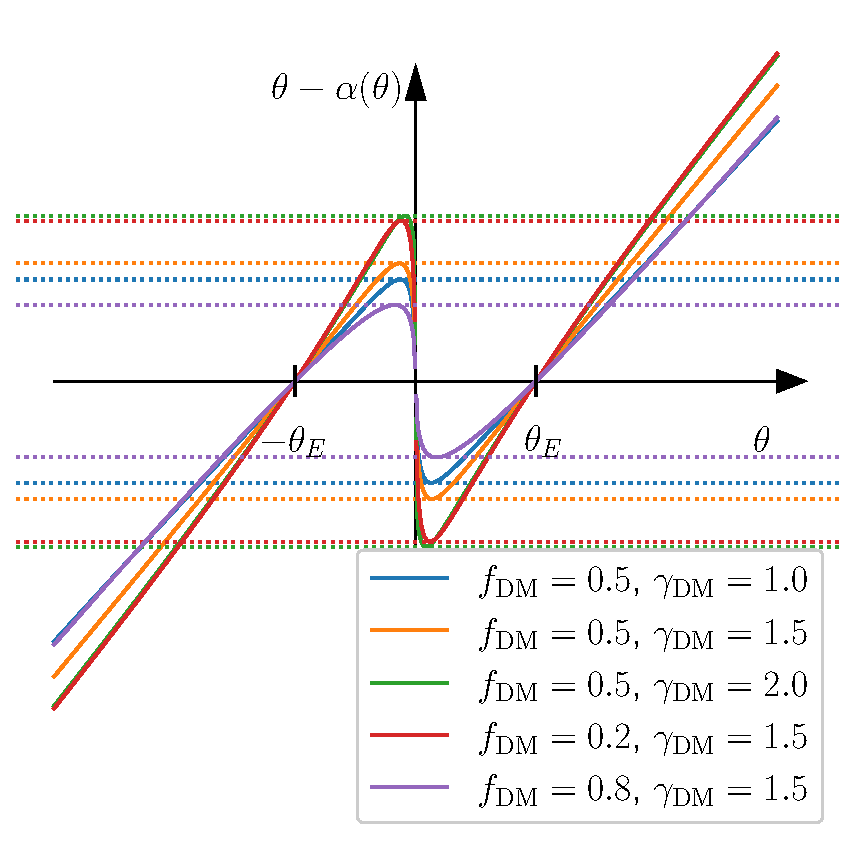
\includegraphics[width=\columnwidth]{composite_fixedap_scheme.eps}
\caption{
The lens equation of axisymmetric lenses. Solid lines: right-hand side of \Eref{eq:1dlenseq} for five lenses with different density profiles. 
Given a source at position $\beta$, its lensed images form at the values of $\theta$ where the solid line intersects a horizontal line located at $\beta$ on the vertical axis. 
Dotted lines: positions of the radial caustics. Sources located within the radial caustic of a given lens produce three images.
The lens models used in this simulations consist of a stellar component and a dark matter halo, as described in section \ref{ssec:profile}. Their density profile is plotted in \Fref{fig:kappa}.
\label{fig:scheme}
}
\end{figure}
%The slope of the $\theta - \alpha(\theta)$ curve is the inverse of the magnification of an image in the radial direction. 
%This can be understood by noting that, according to \Eref{eq:1dlenseq}, the derivative of $\theta - \alpha(\theta)$ is equal to $d\beta/d\theta$, which quantifies the ratio between an infinitesimal displacement in the radial direction in the source plane and the corresponding displacement in the image plane.
%Stationary points of the $\theta - \alpha(\theta)$ curve, therefore, are points of infinite magnification in the radial direction. For a given axisymmetric lens, these points describe a circle known as the radial critical curve. 
%The corresponding curve in the source plane, the radius of which is given by the value of $\theta - \alpha(\theta)$ at the stationary point, is known as the radial caustic.
%As can be seen in \Fref{fig:scheme}, sources that lie within the radial caustic are strongly lensed into three images, while sources that lie outside of it produce only one image.

%Strong lenses also have a tangential critical curve, where the magnification along the tangential direction is formally infinite. For an axisymmetric lens, the tangential critical curve is a circle with radius equal to the Einstein radius, and the corresponding tangential caustic collapses to the $\beta=0$ point in the source plane.

\subsection{The elliptical lens}

In this paper we focus mostly on lens galaxies with elliptical isodensity contours.
Given a surface mass density profile $\Sigma(R)$, a lens with an elliptical mass distribution can be obtained by replacing the radial coordinate with the circularised radius:
\begin{equation}
R \rightarrow \sqrt{qx^2 + \frac{y^2}{q}},
\end{equation}
where $x$ and $y$ are cartesian axes centred on the lens centre, with $x$ pointing towards the major axis, and where $q$ is the minor-to-major axis ratio.

\Fref{fig:ellcaust} shows the source-plane caustics of elliptical lenses with different values of the axis ratio.
The outermost curves are radial caustics, while the inner ones are tangential ones.
%While in the axisymmetric case these are a circle and a point respectively (blue curves), in the elliptical case they are transformed into a 
The most striking difference with respect to the axisymmetric case (blue curves in \Fref{fig:ellcaust}) is the fact that the tangential caustic is transformed from a point into a diamond-like curve.
Sources located within the diamond produce five images (one of which is usually highly de-magnified). Sources that lie in the region enclosed between the two caustics are imaged three times. Sources outside the radial caustic are imaged only once, as in the axisymmetric case.
The fact that the number of images changes by two at a caustic crossing is a general feature of gravitational lenses with no singularities \citep{SEF92}.

\begin{figure}
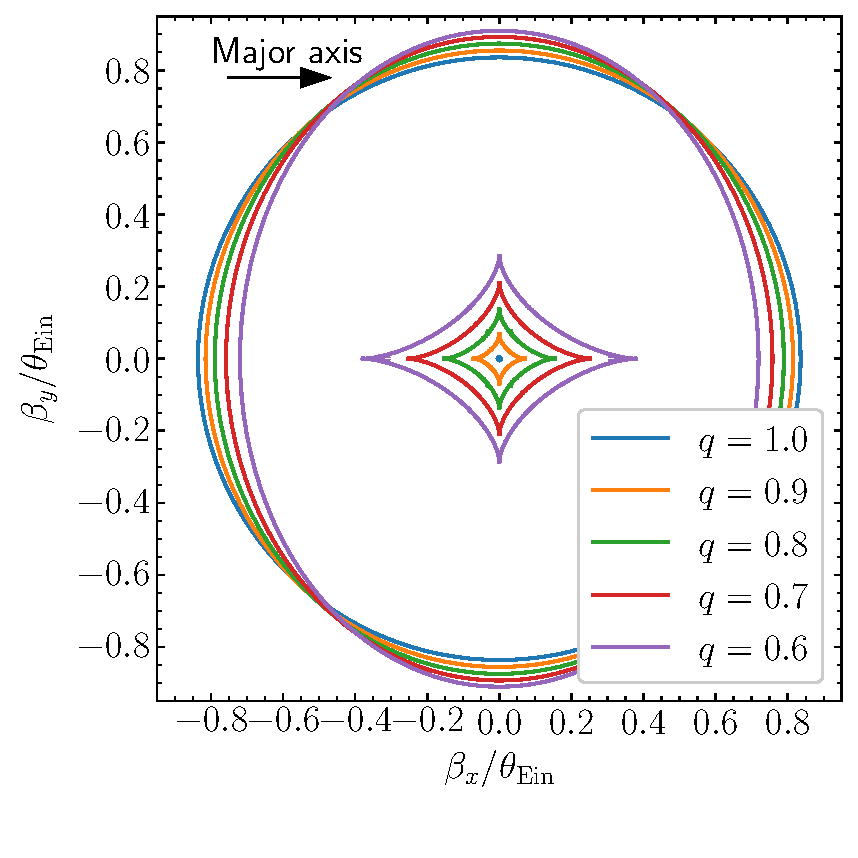
\includegraphics[width=\columnwidth]{composite_caustics.eps}
\caption{
Caustics of lenses with fixed radial structure and different ellipticity.
Source-plane angular coordinates are in units of the Einstein radius.
The outer curve is the radial caustic, while the inner diamond is the tangential caustic. Sources located outside the caustic are not strongly lensed. Sources that lie in the region enclosed between the two caustics produce three images, while sources inside the tangential caustic produce five images.
The lens model adopted for this experiment consists of a stellar component and a dark matter halo, as described in \ref{ssec:profile}. The two components have the same ellipticity.
\label{fig:ellcaust}
}
\end{figure}

\subsection{Lensing event definition: point sources}\label{ssec:lensdefpoint}

In order to compute the probability of a lensing event we must provide an exact definition for it.
A necessary condition for a lens-source system to qualify as a strong lens is the presence of multiple images of the source.
As we showed above, this requires the source to lie within the region enclosed by the radial caustic.
In order to recognise a strong lens in a real strong lensing survey, however, it is not sufficient for multiple images to exist: they must be detected.
For this reason, given the detection limit of a survey for a point source, $m_{\mathrm{lim}}$, we define as strong lensing event any lens-source system with at least two images brighter than $m_{\mathrm{lim}}$.
This is the same definition upon which the \citet{MVK09} work is based \citep{VMK09}.
Labelling with $m_2$ the magnitude of the second-brightest image, then, in the absence of photometric noise the lens detection probability $\pdet$ becomes
\begin{equation}\label{eq:pointdet}
\pdet(\psilens,\psisource) = \left\{\begin{array}{ll} 1 & \rm{if}\,m_2(\psilens,\psisource) < m_{\mathrm{lim}} \\
0 & \rm{otherwise}\end{array}\right. .
\end{equation}

\subsection{Lensing event definition: extended sources}\label{ssec:lensdefext}

Defining a strong lensing event in the case of an extended source is less straightforward.
In principle, we should require parts of the source to be multiply imaged.
In practice, it is not always easy to determine whether a lensed image contains multiple images or not.
This is because, when the source is extended, some of the images can be blended together.
In real strong lensing surveys, it is common to find lens candidates in which the lensed source consists only a single arc. In those cases it is difficult to establish whether the arc is a set of blending images or not, and the decision of including such systems in a strong lens sample is often arbitrary.
%For instance, a source located on one of the cusps of a tangential caustic produces a merging set of three magnified images. If the source is extended and no counter-image is detected, however, the appearence of the merging triplet is very similar to that of a single arc with no multiple images, and it can be difficult to differentiate between the two cases.
%In real strong lensing surveys, the decision of including systems with a single arc or not is often arbitrary.

For the purpose of carrying out our experiment we adopt the following definition. First, we determine the footprint of the lensed source. We define this as the ensemble of pixels where the source is detected with $S/N>2$. The footprint is in general composed of multiple disconnected regions, corresponding to the different images. In order to only include images that can be clearly identified, we add the condition that the integrated $S/N$ of each separate region must be $S/N > 10$. This condition has the effect of removing from the source footprint any isolated region consisting only of a very small number of pixels. In a real-world application, it would be very hard to classify such marginal detections as images.
If, after applying this cut, the source footprint is spread over multiple separated regions, then the system is classified as a lens.
Additionally, if the source footprint consists of only a single region, we still classify it as strongly lensed if it subtends an angle larger than $90^\circ$ measured from the lens centre. This last criterion allows us to include highly magnified arcs and full rings.

%Additionally, we classify as strongly lensed the following set of sources any full rings, and any single arcs that subtend an angle larger than $90^\circ$ measured from the lens centre. This last criterion is a 
%Additionally, we classify as a strongly lensed source any full rings, and any single arcs that subtend an angle larger than $90^\circ$ measured from the lens centre. This last criterion is a 

%Given the source footprint thus defined, we classify the system as a strong lens if the footprint subtends an angle $\theta_{\mathrm{s}}$ with respect to the lens centre that satisfies the following condition:
%Given the source footprint thus defined, we classify the system as a strong lens if we can find two points on the footprint that subtend an angle $\theta_{\mathrm{s}}$ with respect to the lens centre that satisfies the following condition:
%\begin{equation}\label{eq:subtend}
%\theta_{\mathrm{min}} < \theta_{\mathrm{s}} \leq 180^\circ,
%\end{equation}
%with $\theta_{\mathrm{min}}=90^\circ$.
%A similar criterion was used in the automatic lens search campaign of \citet{Son++18a}.

\Fref{fig:lensdef} shows a few examples of how this criterion can be used to classify lenses.
As the first three examples in \Fref{fig:lensdef} show, the presence of multiple images or a full ring implies that the system is classified as a lens. Only if the source footprint subtends an angle smaller than $90^\circ$, a system is not considered a strong lens (fourth example).
%The choice of points used to define the angle $\theta_{\mathrm{s}}$ is not unique: any pair of points for which \Eref{eq:subtend} is satisfied is acceptable.

\begin{figure*}
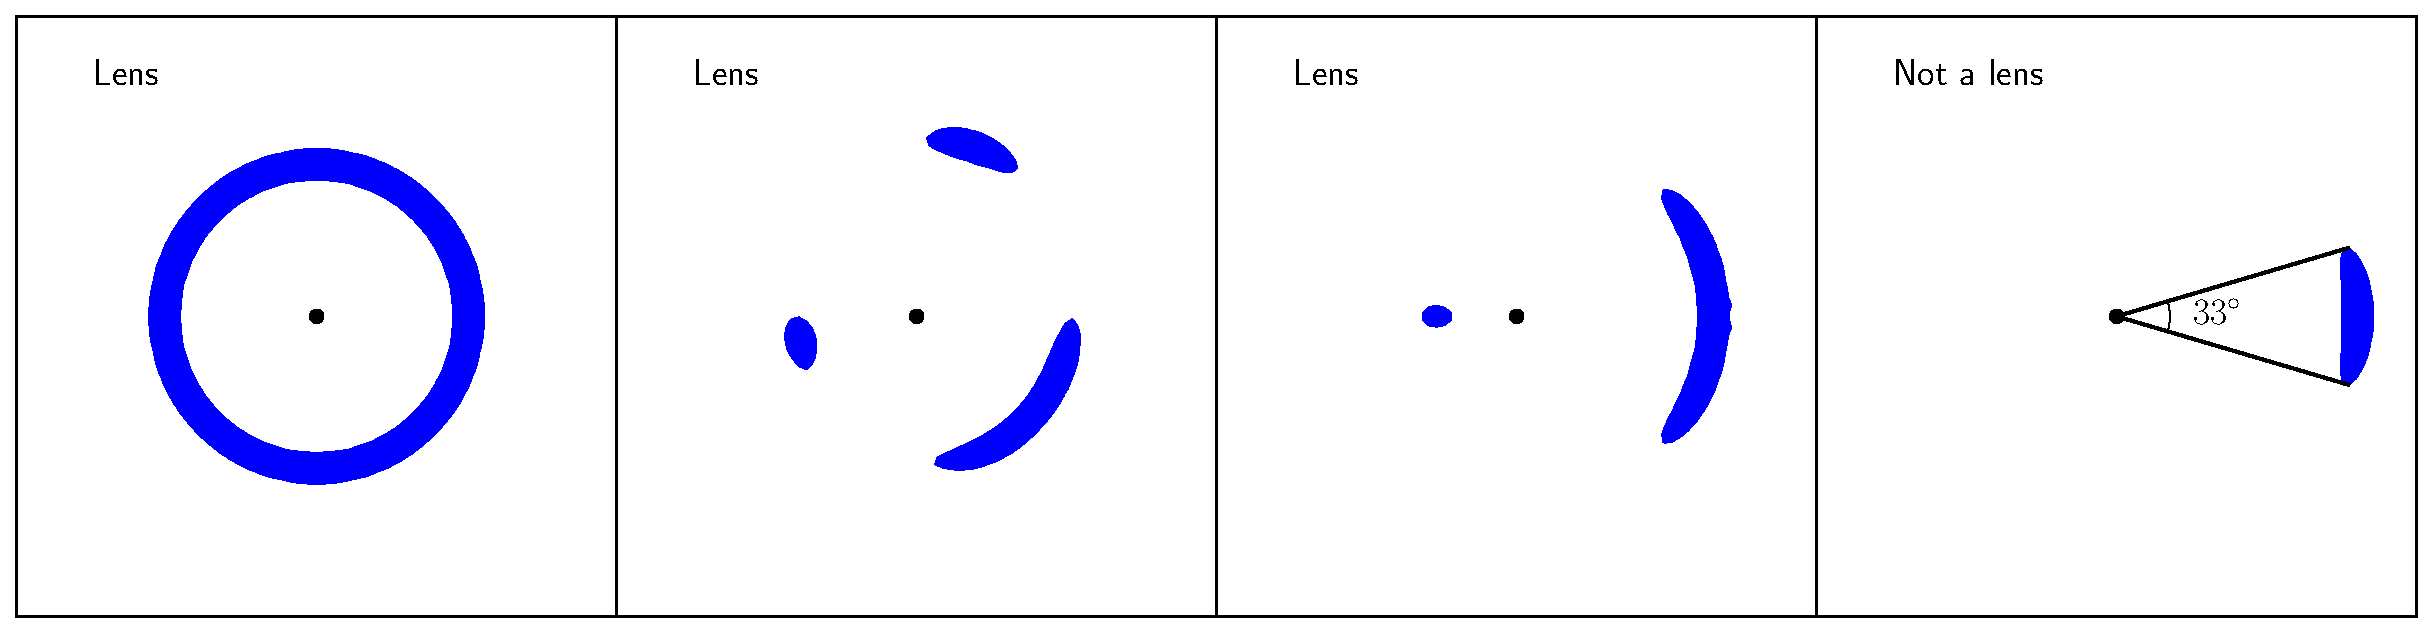
\includegraphics[width=\textwidth]{footprints.eps}
\caption{
Criterion used to classify lensed images of extended sources. Four examples. In each panel, the blue regions are the footprint of the lensed source. 
The two segments connecting the source footprint to the lens centre show the largest angle subtended by the source. If this angle is larger than $90^\circ$, the system is classified as a strong lens.
\label{fig:lensdef}
}
\end{figure*}
%__________________________________________________________________

\section{Individual lenses}\label{sect:indlenses}

In this section we study how the probability of a strong lensing event varies as a function of lens and source properties.
In order to do so, it is useful to introduce the concept of strong lensing cross-section.
Given a foreground galaxy with parameters $\psilens$, a background source with parameters $\psisource$, and a criterion $S$ to define a strong lensing event, the strong lensing cross-section is defined as \citep{Son22}:
\begin{equation}\label{eq:crosssect}
\crosssect = \int_{\mathbb{R}^2} d\boldsymbol\beta \pdet(\psilens,\psisourcenobeta,\boldsymbol\beta|S),
\end{equation}
where $\boldsymbol\beta$ is the position of the background source, $\psisourcenobeta$ is the ensemble of source parameter except for the position, and the integral is carried out over the whole sky.
The definition above is valid for both a point source and an extended source: although there is no unique way of defining the position of an extended source, the integral over the sky ensures that the result is independent of how the source position is defined.
In the limit of low density of background sources, which is satisfied in all practical cases, the probability of a lensing event is proportional to $\crosssect$.

We compute $\crosssect$ in a series of different scenarios of increasing complexity.
%We first introduce the basic equations of gravitational lensing in section \ref{ssec:lensbasics}.
%Then, in section \ref{ssec:profile}, we present the model family adopted to describe the radial density profile of the lenses in our experiments.
The model family adopted to describe the radial density profile of the lenses is the same in all of our experiments. We describe this in section \ref{ssec:profile}. %, among with the basic equations of gravitational lensing.
%In section \ref{ssec:axsymmpoint} we consider axisymmetric lenses and point sources.
In section \ref{ssec:axsymmpoint} we show calculations of the strong lensing cross-section in the case of axisymmetric lenses and point sources.
In section \ref{ssec:ellpoint} we generalise the lens geometry to elliptical, while in section \ref{ssec:ellext} we replace point sources with extended sources.

%\subsection{Strong lensing basics}\label{ssec:lensbasics}


\subsection{Lens density profile}\label{ssec:profile}

Throughout this work we describe the mass distribution of the lens galaxies with a two-component model consisting of a S\'{e}rsic profile, describing the baryonic component of a galaxy, and a generalised Navarro, Frenk \& White (gNFW) profile, describing the dark matter halo.
We assume that the two components are concentric.
We also assume that the baryonic component consists entirely of stars.
This is a good approximation for the majority of the known strong lenses, which are massive elliptical galaxies with little gas.
Finally, we assume that the light distribution of the stellar component follows its mass distribution exactly. That is, we do not allow for the presence of gradients in the stellar mass-to-light ratio. This assumption is probably broken in real galaxies but, as we discuss in \Sref{sect:discuss}, does not impact our investigation.

%Lensing-related quantities depend on the projected mass distribution $\Sigma(R)$.
%For the purpose of computing lensing-related quantities, the projected massdistribution $\Sigma(R)$ is needed.
%For a S\'{e}rsic profile, this is given by
The projected surface mass density of a S\'{e}rsic profile is given by
\begin{equation}
\Sigma(R) = \Sigma_0 \exp{\left\{-b\left(\frac{R}{\reff}\right)^{1/4}\right\}},
\end{equation}
with
\begin{equation}
\Sigma_0 = \frac{\mstar b^{2n}}{2\pi n \reff^2 \Gamma(2n)},
\end{equation}
where $\mstar$ is the total mass, $\reff$ is the radius enclosing half of the total mass, $n$ is the S\'{e}rsic index, $\Gamma$ is the incomplete Gamma function, and $b$ is given by \citep{C+B99}
\begin{equation}
b(n) \approx 2n -\frac13 + \frac{4}{405n} + \frac{46}{25515n^2} + O(n^{-3}).
\end{equation}
Throughout this paper we indicate with $\teff$ the angular size of the half-light radius.

The dark matter component is first defined by means of its three-dimensional distribution, which for a spherically symmetric gNFW profile is
\begin{equation}
\rho(r) = \dfrac{\rho_0}{(r/r_s)^{\gammadm}\left(1 + r/r_s\right)^{3-\gammadm}}.
\end{equation}
The parameter $\gammadm$ is the inner density slope, $\rho_0$ is a normalisation parameter, while $r_s$ is the scale radius. The logarithmic slope of the density profile transitions from $-\gammadm$ to $-3$ at a radius $r\approx r_s$.
The projected surface mass density of a gNFW profile can be expressed in terms of the following integral \citep{WTS01}:
\begin{equation}
\Sigma(R) = 2r_s\rho_0 \left(\frac{R}{r_s}\right)^{1-\gammadm}\int_0^{\pi/2} dx \sin{x}(\sin{x} + R/r_s)^{\gammadm-3}.
\end{equation}

\Fref{fig:kappa} shows the dimensionless surface mass density profile of S\'{e}rsic + gNFW models with various values of the inner dark matter density slope $\gammadm$ and of the fraction of projected dark matter mass within the half-light radius, $\fdm$.
All of the profiles have a S\'{e}rsic index $n=4$, a dark matter scale radius equal to ten times $\reff$, and are normalised in such a way that the Einstein radius is equal to the half-mass radius of the stellar component. 
Two main features emerge from \Fref{fig:kappa}. First, the baryons generally dominate the total density in the inner regions $(\theta < \tein)$, while the dark matter is the main component at large radii.
Second, models with different dark matter fractions and inner dark matter slopes can conspire to produce very similar total density profiles. 
%it is possible to build models with different dark matter fractions and inner dark matter slopes, but with very similar total density profiles. 
This is the case, for example, of the ($\fdm=0.5,\gammadm=1.5$) and the ($\fdm=0.2,\gammadm=2.0$) models (green and blue lines in \Fref{fig:kappa}).

%
\begin{figure}
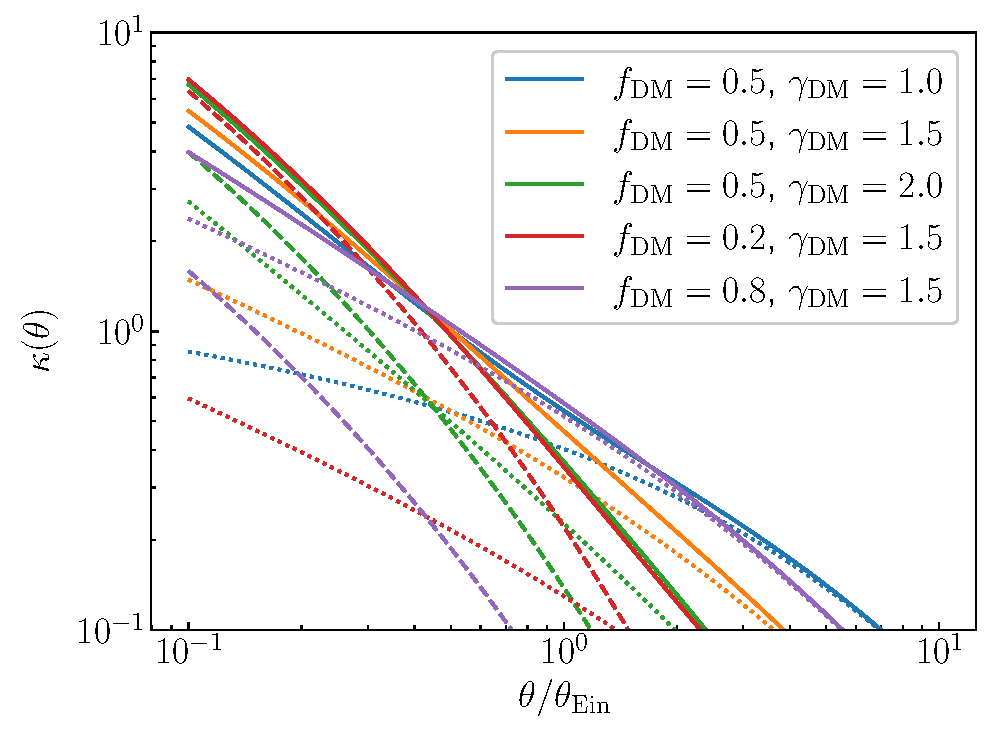
\includegraphics[width=\columnwidth]{composite_fixedap_kappa.eps}
\caption{
Dimensionless surface mass density profile of S\'{e}rsic + gNFW composite models.
The S\'{e}rsic index of the baryonic component is fixed to $n=4$ and the scale radius of the dark matter component is fixed to ten times the half-light radius.
All of the profiles are normalised in such a way that the Einstein radius is equal to the half-light radius.
Solid lines: total density profile. Dotted lines: dark matter density profile. Dashed lines: baryonic density profile.
The blue, orange and green dashed lines are identical, as they correspond to profiles with the same fraction of baryonic mass within the half-light radius.
\label{fig:kappa}
}
\end{figure}
%

\subsection{Axisymmetric lenses, point sources}\label{ssec:axsymmpoint}

Axisymmetric lenses with a density profile of the kind introduced in section \ref{ssec:profile} can produce either one or three images of a point source.
This can be seen in \Fref{fig:scheme}, which shows the lens equation for various values of the dark matter fraction and the inner dark matter slope.
All of the lenses shown in this figure have the same Einstein radius, which is equal in size to the half-mass radius of the stellar component.
The radius of the radial caustic, marked by the dotted lines in \Fref{fig:scheme}, is a strong function of the lens properties: it is largest in lenses with a smaller dark matter fraction or steeper dark matter slopes.
As a result, the source plane area that is subject to strong lensing is an even stronger function of these properties, since it scales with the square of the radial caustic radius.
In order to compute the lensing cross-section, however, we must take into account the magnification of the multiple images: according to our definition of a strong lensing event, given in section \ref{ssec:lensdefpoint}, at least two images must be detected in order for a system to qualify as a strong lens.

\Fref{fig:1dmag} shows the magnification of the secondary image as a function of source position. The secondary image is the one located in the region between the radial and tangential critical curves, opposite to the source with respect to the lens centre. In most practical cases this is the second brightest image.
As \Fref{fig:1dmag} shows, the magnification is very large for sources close to the lens (small values of $\beta$), decreases with increasing source position and then increases in close proximity to the radial caustic.
%In particular, for $\beta > 0.5\tein$, the magnification is smaller than unity, with the exception of a thin slice near the caustic.
While for the model with $f_{\mathrm{DM}}=0.8$ (purple curve) the magnification is above unity everywhere, other lens models can produce highly de-magnified secondary images for large values of $\beta$.
Depending on the intrinsic brightness of the lensed source, these images may or may not be detected.
%This has two implications for the lensing cross-section. First, a larger caustic size does not necessarily translate into a larger value of $\crosssect$. Second, the cross-section depends on the intrinsic brightness of the lensed source: an extremely bright point source can be detected regardless of its position in the source plane, but a source with a finite brightness can go undetected depending on its value of $\beta$.

%
\begin{figure}
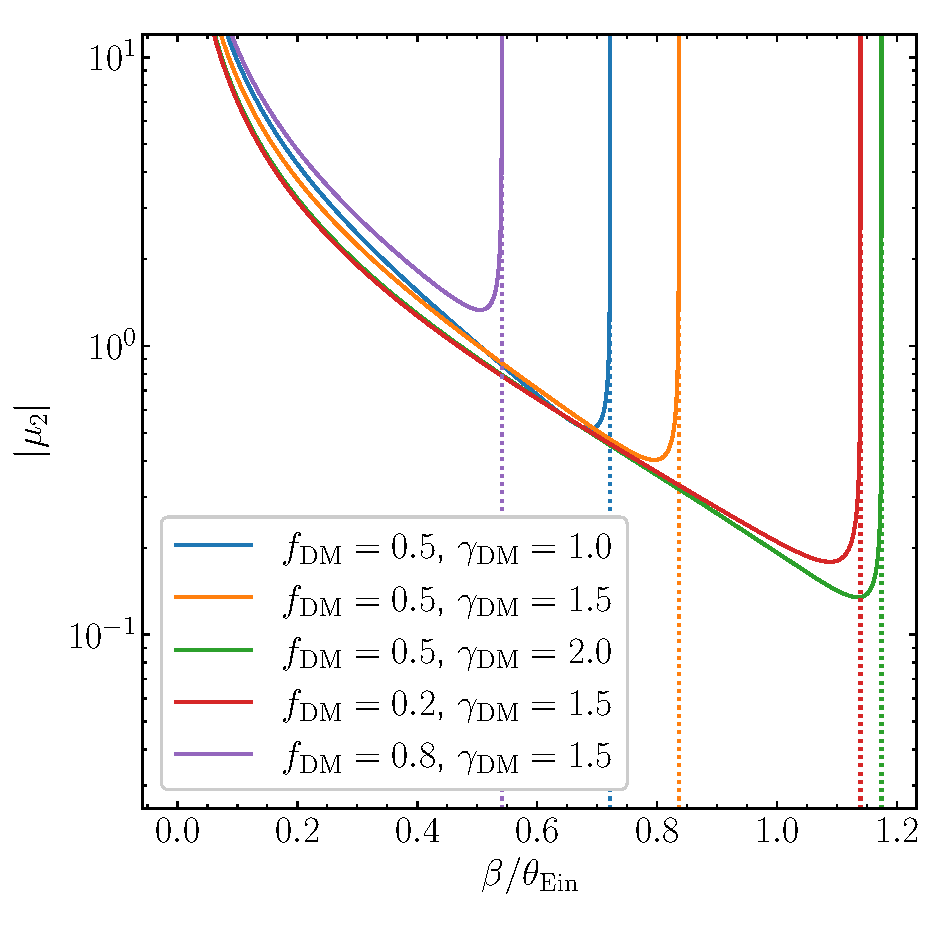
\includegraphics[width=\columnwidth]{composite_fixedap_mu2.eps}
\caption{
Magnification of the secondary image as a function of the source position.
The lenses are axisymmetric composite model. Their density profile is plotted in \Fref{fig:kappa}.
Vertical dotted lines mark the position of the radial caustic.
\label{fig:1dmag}
}
\end{figure}

Using the definition of \Eref{eq:crosssect}, we computed the lensing cross-section of a set of axisymmetric lenses, with respect to point sources with different brightnesses.
In particular, we considered model lenses with fixed Einstein radius, with angular half-mass radius $\teff$ fixed to $\tein$, and varying values of the dark matter fraction and dark matter inner slope.
The results are shown in \Fref{fig:fixedap_cs}.
Each line corresponds to a source with a given intrinsic (i.e. unlensed) magnitude, $m_s$. The difference between this magnitude and the limiting magnitude of the survey is indicated as follows:
\begin{equation}
\Delta m \equiv m_s - m_{\mathrm{lim}}.
\end{equation}

We can see a clear trend between $\Delta m$ and the lensing cross-section, in both panels of \Fref{fig:fixedap_cs}: $\crosssect$ is larger for brighter sources.
The trend saturates below a certain $\Delta m$, for sufficiently small values of $\gammadm$ or for sufficiently large values of $\fdm$.
%These are cases in which the source is so bright that, as long as it is located within the radial caustic, it always produces at least two detectable images. 
In these cases the lensing cross-section coincides with the full area enclosed within the caustic, and further increasing the source brightness does not result in an increased value of $\crosssect$.

\begin{figure}
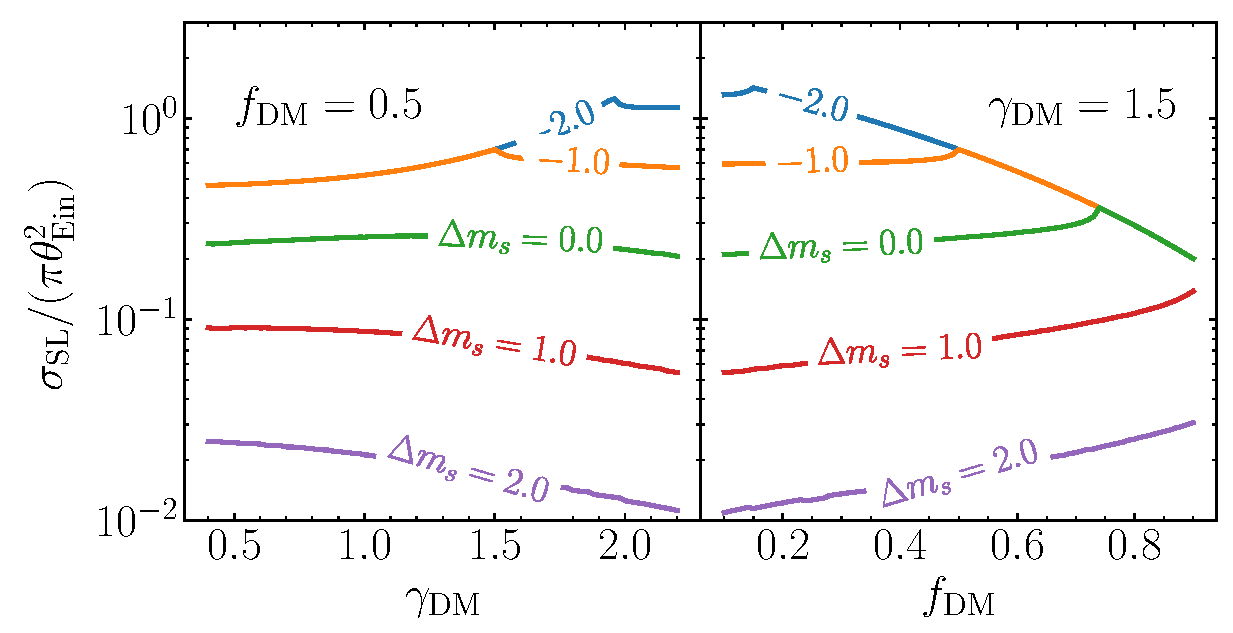
\includegraphics[width=\columnwidth]{axisymm_composite_crosssect.eps}
\caption{
Strong lensing cross-section of an axisymmetric lens and a point source.
The lens galaxy is a composite model, introduced in section \ref{ssec:profile}, with angular half-light radius equal to the Einstein radius.
Left panel: cross-section, in units of $\pi\tein^2$, as a function of the inner dark matter slope. The dark matter fraction is fixed at $\fdm=0.5$.
Right panel: cross-section as a function of the fraction of dark matter within the half-light radius. The inner dark matter slope is fixed at $\gammadm=1.5$.
The system is defined as a strong lens if at least two images are detected.
Different lines correspond to the difference $\Delta m$ between the source magnitude and the survey detection limit for a point source.
\label{fig:fixedap_cs}
}
\end{figure}

At fixed source brightness, trends with the dark matter inner slope or dark matter fraction are generally weak.
The lines of \Fref{fig:fixedap_cs}, however, have been computed by keeping the Einstein radius fixed while varying $\gammadm$ or $\fdm$.
This is achieved by adjusting other properties of the lens, such as the total mass of the baryonic or the dark matter component (see \Fref{fig:kappa}). 
%This means that other properties of the lens, such as the total mass of the baryonic component or the dark matter component, are adjusted to maintain a constant $\tein$ (see \Fref{fig:kappa}). 
In practice, when varying one ingredient of the lens density profile, the Einstein radius varies in response.
To get a complete view of how the lensing cross-section depends on different lens properties, we also computed how $\crosssect$ responds in absolute terms by varying one lens parameter at a time.
\Fref{fig:phys_cs} shows $\crosssect$ as a function of stellar mass, half-light radius, inner dark matter slope, and projected dark matter mass enclosed within an aperture of $5$~kpc, $\mdmfive$.
%The reference lens is a galaxy at $z=0.3$ with $\log{\mstar}=11.5$, $\reff=7\,{\rm kpc}$, $\gammadm=1.5$, $\log{\mfive}=11.0$, and a source at $z=1.5$.

\begin{figure*}
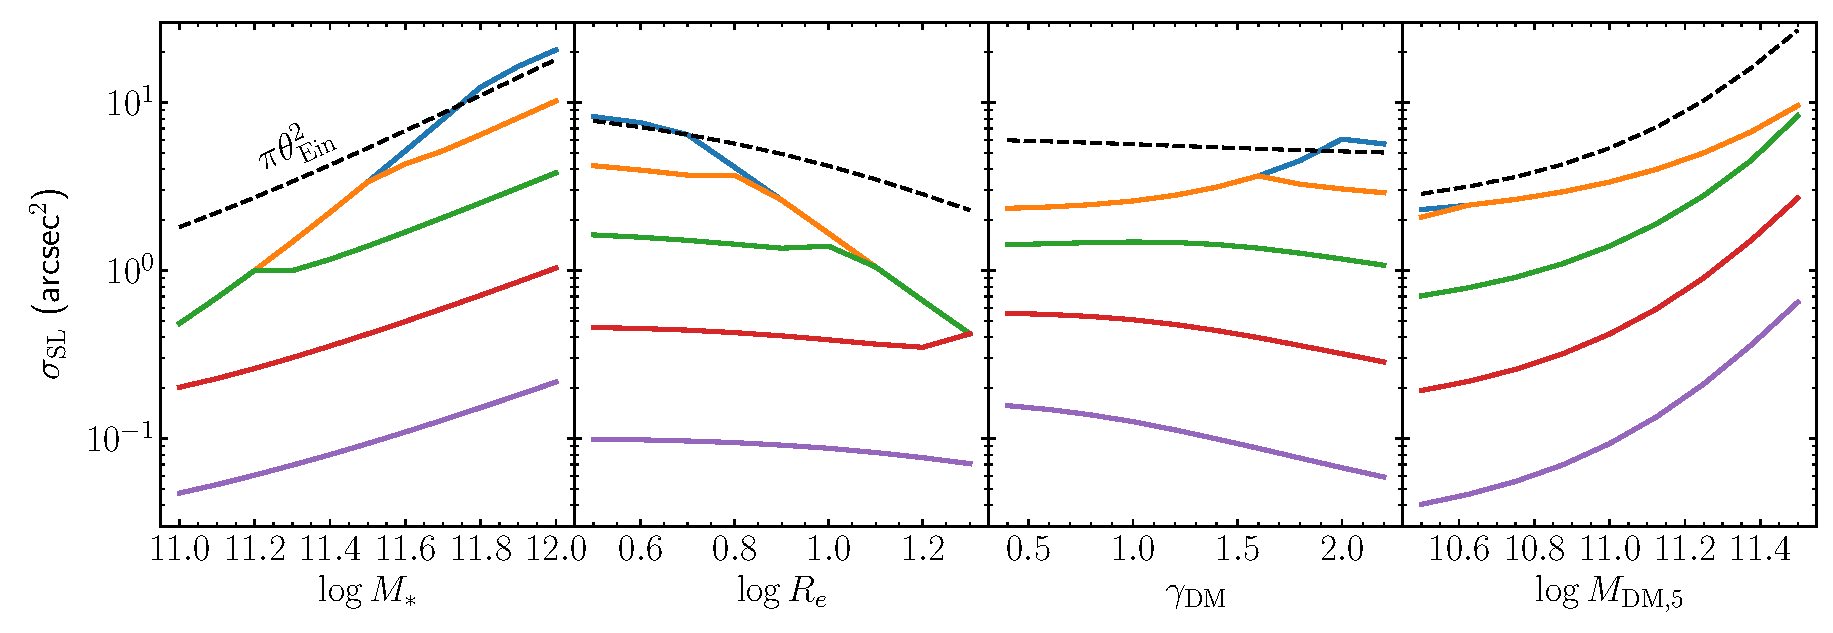
\includegraphics[width=\textwidth]{axisymm_composite_physical_crosssect.eps}
\caption{
Absolute value of the strong lensing cross-section as a function of various lens properties.
The reference lens is a galaxy at $z=0.3$ with $\log{\mstar}=11.5$, $\reff=7\,{\rm kpc}$, $\gammadm=1.5$, $\log{\mdmfive}=11.0$, $r_s=100$~kpc, and a source at $z=1.5$
In each panel, only one property of the lens is varied, as indicated on the label of the horizontal axis.
Each curve corresponds to a different value of $\Delta m$, in accordance with \Fref{fig:fixedap_cs}.
The dashed line in each panel shows the quantity $\pi\tein^2$.
\label{fig:phys_cs}
}
\end{figure*}

The lensing cross-section increases with increasing stellar mass and dark matter mass, decreases with increasing $\reff$ for bright sources, while is only a weak function of $\gammadm$. 
The lack of a clear trend between $\crosssect$ and $\gammadm$ appears to be in contradiction with the result of \citet{MVK09}, who found a strong positive correlation between $\crosssect$ and $\gammadm$.
The origin of this discrepancy lies in the different ways in which $\gammadm$ is varied in the two experiments. While we varied $\gammadm$ at fixed $\mdmfive$, \citet{MVK09} kept fixed the virial mass of the dark matter halo. At fixed virial mass, increasing the inner dark matter slope results in a correspondingly larger dark matter mass in the inner regions, which naturally results in a larger lensing cross-section.

\Fref{fig:fixedap_cs} and \Fref{fig:phys_cs} show that the trends between lens properties and the strong lensing cross-section can be different for sources with different brightnesses.
The net effect in a strong lensing survey is an average over the source population, weighted by the source luminosity function. 
This implies that surveys that target different families of sources, with different luminosity functions (for instance, galaxies or quasars), can have different strong lensing biases. We explore this possibility in \Sref{sect:lenspop}.

\subsection{Elliptical lenses, point sources}\label{ssec:ellpoint}

We measured $\crosssect$ for lenses with a fixed radial density profile and different ellipticities, with respect to point sources of diferent brightnesses.
%In particular, we took a lens at redshift $z_{\mathrm{l}}=0.3$, with $\log{\mstar}=11.5$, $\reff=7$~kpc, $\log{\mdmfive}=11.0$, $r_s=100$~kpc, $\gammadm=1.5$, and a source at redshift $z_{\mathrm{s}}=1.5$. 
%In particular, we took a lens at redshift $z_{\mathrm{l}}=0.3$, with $\log{\mstar}=11.19$, $\reff=4.45$~kpc, $\fdm=0.5$, $r_s=100$~kpc, $\gammadm=1.5$, and a source at redshift $z_{\mathrm{s}}=1.5$. This corresponds to a lens with Einstein radius equal to the half-light radius, both equal to $1''$.
In particular, we set $\fdm=0.5$, $\gammadm=1.5$, $r_s=10\reff$, $\tein=\teff$, and set the ellipticities of both the baryonic and dark matter components to be the same, with the same orientation of the major axis.
This is the lens model used to produce the caustics plot of \Fref{fig:ellcaust}.
That figure suggests that the size of the source plane area subject to strong lensing, the area enclosed within the outermost caustic, does not vary strongly with the ellipticity of the lens.
Therefore we expect the strong lensing cross-section to be a weak function of ellipticity.

We carried out the computation of $\crosssect$ by means of simulation: we generated a large number of point sources over a given area that includes the caustic, then used the software {\sc Glafic} \citep{Ogu21} to solve the lens equation, find the number of images and their magnification. We then multiplied the area over which sources are located by the fraction of those that are strongly lensed according to the criterion of \Eref{eq:pointdet}.
%\Fref{fig:ellcaust} suggests that the size of the source plane area subject to strong lensing, the area enclosed within the outermost caustic, does not vary strongly with the ellipticity of the lens.
%Therefore we expect the strong lensing cross-section to be a weak function of ellipticity.
The resulting $\crosssect$ is shown in \Fref{fig:ellpoint_cs} as a function of the minor-to-major axis ratio $q$.

\begin{figure}
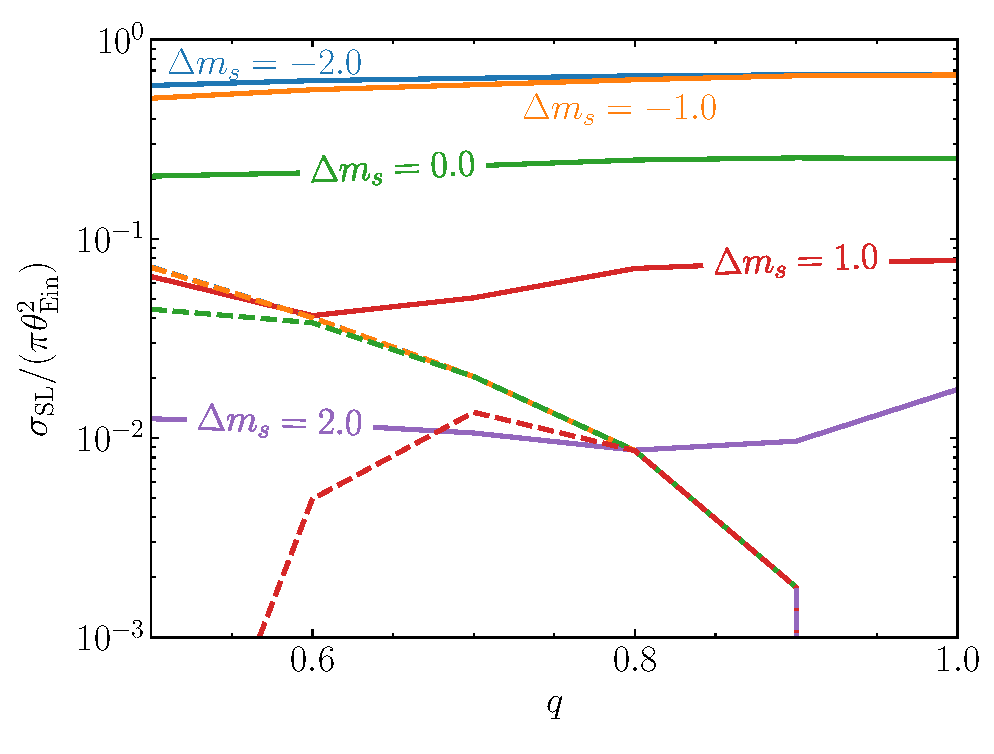
\includegraphics[width=\columnwidth]{ell_pnt_cs.eps}
\caption{
Point source strong lensing cross-section as a function of lens axis ratio.
Solid lines: cross-section based on the lens event definition of \Eref{eq:pointdet}.
Dashed lines: cross-section based on the detection of four images (quad cross-section).
Lines of different colour correspond to sources of different intrinsic magnitude.
%The lens consists of a galaxy at redshift $z_{\mathrm{l}}=0.3$, with $\log{\mstar}=11.19$, $\reff=4.45$~kpc, $\fdm=0.5$, $r_s=100$~kpc, $\gammadm=1.5$, and a source at redshift $z_{\mathrm{s}}=1.5$.
The parameters of the lens density profile are $\fdm=0.5$, $\gammadm=1.5$, $r_s=10\reff$, $\teff=\tein$.
The baryonic and dark matter components have the same ellipticity and direction of the major axis.
\label{fig:ellpoint_cs}
}
\end{figure}

For bright sources the strong lensing cross-section is approximately constant with axis ratio. This is because, as pointed out earlier, in the bright source regime the cross-section is determined by the area enclosed within the radial caustic, which does not vary much with lens ellipticity.
For faint sources we observe a larger variation with $q$, with a factor of two difference between the largest and smallest value of $\crosssect$ at fixed source brightness.

Most of the sources that result in detectable lenses produce two detectable images. These are sources that are located in the region enclosed bewteen the radial and the tangential caustic. 
%In most cases, only two of these three images are detected: the third one, close to the centre, is usually highly de-magnified.
If the source is located within the tangential caustic, however, four detectable images are usually created.
Lenses with four visible images, usually referred to as quad lenses, are sometimes given a high priority in certain lensing studies, because they offer more constraints compared to double lenses. For instance, quads make up the majority of the lenses used so far in time-delay studies \citep{Mil++20}.
For this reason we also computed an alternative lensing cross-section, in which the definition of a lensing event requires the detection of four images, instead of two.
This is plotted in \Fref{fig:ellpoint_cs} with dashed lines.
The cross-section for quads is a strong function of lens ellipticity, for bright sources.
This is a consequence of the fact that the area enclosed within the tangential caustic, which is where a source needs to be in order to produce four images, increases with increased lens ellipticity, as \Fref{fig:ellcaust} shows.
For sources that are intrinsically fainter than the detection limit, however, the quad cross-section is extremely small.


\subsection{Elliptical lenses, extended sources}\label{ssec:ellext}

In the case of an extended source, the complexity of the problem is increased due to the addition of a series of features: the surface brightness distribution with its radial profile, shape and orientation, and the point spread function (PSF). 
For the sake of reducing the dimensionality of the problem, we neglected the PSF and focus on circularly symmetric sources. We also fixed the surface brightness profile to an exponential disk (i.e. a S\'{e}rsic model with $n=1$).
We then took a lens model with the same parameters used in section \ref{ssec:ellpoint} and a minor-to-major axis ratio of $q=0.7$.
We created a grid of pixels with $0.05''$ size, then computed the lensing cross-section by simulating a large number of images of extended sources with {\sc Glafic} and measuring the fraction of them that results in a strong lens, according to the definition of section \ref{ssec:lensdefext}.
We carried out experiments with sources with different values of the total flux and varying half-light radius, $\theta_{\mathrm{e,s}}$.
The results are shown in \Fref{fig:extcs}.
The total flux of the source, indicated in the legend, is measured in units of the sky background fluctuation within an area equal to the square of the Einstein radius. We assumed that the background noise is an uncorrelated Gaussian field, for this purpose.

\begin{figure}
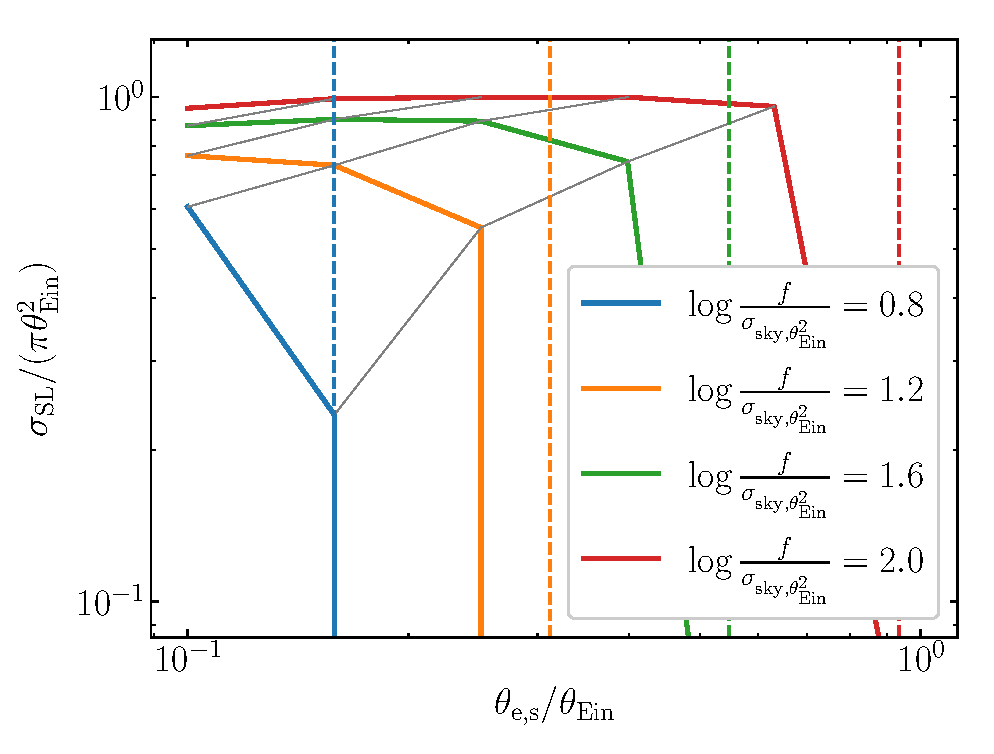
\includegraphics[width=\columnwidth]{ell_ext_cs.eps}
\caption{
Strong lensing cross-section as a function of source half-light radius.
The lens model is the same as in \Fref{fig:ellpoint_cs}, with axis ratio $q=0.7$. The source is a circular exponential profile.
Each solid line corresponds to a different value of the total flux of the source. The flux $f$ is expressed in terms of the background noise fluctuation measured over an area equal to $\tein^2$.
The vertical dashed lines correspond to the maximum size for which a galaxy with a given flux can be detected in the absence of lensing.
%Solid grey curves are lines of constant effective surface brightness, $f/(2\pi\theta_s^2)$.
\label{fig:extcs}
}
\end{figure}

As in the point source case, the lensing cross-section increases with increasing total flux, at fixed source size.
At fixed flux, $\crosssect$ stays approximately constant with increasing source size until a given value, then drops rapidly for larger sizes.
From a qualitative point of view, this behaviour can be observed also in the absence of lensing: increasing the size of a galaxy while keeping its flux fixed lowers its average surface brightness. If the surface brightness drops below the sky fluctuation level, then it becomes very difficult to detect it.
In order to determine whether there are lensing-specific features in the $\crosssect-\theta_{\mathrm{e,s}}$ relation of \Fref{fig:extcs}, we computed, for each source flux, the maximum half-light radius for which it can be detected in the absence of lensing.
We used the same criterion as that of section \ref{ssec:lensdefext} to define a detection: we defined the source footprint as the ensemble of pixels that are $2\sigma$ above the background and required the total signal-to-noise ratio within the footprint to be larger than ten.
The resulting limiting sizes are shown as vertical lines in \Fref{fig:extcs}. For each given total flux, the non-lensing size limit is similar to the value of $\theta_{\mathrm{e,s}}$ at which the lensing cross-section drops.

This result suggests that, to first approximation, lensing does not introduce a strong selection in source size.
This is expected, since gravitational lensing preserves surface brightness: a source that can be detected in the absence of lensing will produce images with the same surface brightness when lensed, which can be detected as well.
%When the source is extended, however, 
In order to classify a source as strongly lensed, however, we require that multiple images are observed. 
Only sources that lie within a well-defined region give rise to a strong lensing configuration.
If part of the source extends outside of this region, then only a fraction of its flux contributes to creating a set of strongly lensed images.
This lowers the signal-to-noise ratio of the multiple images compared to the point source case.
%The result is the decrease in $\crosssect$ at values of the source size smaller than the 
The result is that $\crosssect$ starts to decrease with increasing source size at values of $\theta_{\mathrm{e,s}}$ that are smaller than the no-lensing detection limit, as observed in \Fref{fig:extcs}.

%At the brightest flux explored in the experiment (red line in \Fref{fig:extcs}), $\crosssect$ increases with increasing source size, before dropping to zero.
At the brightest flux explored in the experiment (red line in \Fref{fig:extcs}), the lensing cross-section at small source sizes is larger than the area enclosed within the radial caustic (red ellipse in \Fref{fig:cs}).
This is because, when the source is very bright, it can give rise to multiple images even while its centroid lies outside of the radial caustic, as long as its surface brightness distribution extends into it.
This also explains why $\crosssect$ increases with increasing source size, before dropping to zero: the more extended the source, the farther away from the lens centre it can be while still producing multiple images.

%The limit posed by lensing to the maximum detectable source size can be understood as follows.
%In the point source case, at a given flux, only sources that produce at least two images with a sufficiently high magnification are classified as strongly lensed.
%In most practical cases, the limiting factor is the magnification of the secondary image, $\mu_2$, which is a strong function of the source position (see \Fref{fig:1dmag}).
%Only sources that lie within a region of large $\mu_2$, the area of which is equal to the strong lensing cross-section, give rise to a strong lens configuration.
%When the source is extended, different parts of it are magnified by different amounts. If the source size is comparable to or larger than the region of high magnification, then its net magnification averaged over its extent will be lower than in the point-source case, and the secondary image will drop below the detection limit.
%This effect adds to the limit on the source surface brightness in the absence of lensing to produce the trend observed in \Fref{fig:extcs}.

%In the point source case, the necessary and sufficient condition for a source to be strongly lensed is that two detectable images are produced.
%The detection limit of the survey and the intrinsic flux of the source set a requirement on the minimum magnification that two images of the source must have in order for them to be detected.
%The limiting factor is set by the magnification of the secondary image: given a source flux, 
%In the point source case, at a given flux, only sources that lie within a certain region give rise to at least two detectable images, which are required to classify a system as a strong lens. 
%The extent of this region, which is equal to the strong lensing cross-section, is determined by the magnification required in order for the secondary image to be detected (see \Fref{fig:1dmag}).
%The area of this region is equal to the strong lensing cross-section, and decreases for fainter sources. 




%__________________________________________________________________

\section{Lens populations simulations}\label{sect:lenspop}

In the previous section we studied how the lensing cross-section, which is closely related to the term $\pdet$ in \Eref{eq:one}, varies as a function of lens and source properties.
From here on we study the effect that those trends have on populations of lenses.
We do this by simulating populations of foreground galaxies and background sources, selecting strong lenses among them, and comparing the properties of the strong lens sample with the general galaxy population.
Our simulations are based on empirical models, in which existing observations of the baryonic component of galaxies are complemented with a set of assumptions on the mass distribution of the lenses.
In section \ref{ssec:lenses} we explain how we built our foreground galaxy sample,
while in section \ref{ssec:sources} we describe the simulation of the background source population.
In section \ref{ssec:obs} we describe how our mock observations of lenses are generated.

%As we explained in \Sref{sect:intro}, a key ingredient determining the amplitude of the strong lensing bias is the scatter in the mass properties of the foreground galaxy population.
%Although we do not have robust measurements of the intrinsic scatter in properties such as the stellar mass-to-light ratio or the dark matter halo mass, we set upper limits on their amplitude using the 
%Our simulations explore different amplitudes of the scatter. Scatter


%In section \ref{ssec:lenses} we explain how we built our foreground galaxy sample.
%In section \ref{ssec:

\subsection{Foreground galaxies}\label{ssec:lenses}

Our foreground galaxy population consists of a volume-limited sample of early-type galaxies, complete above a minimum observed stellar mass of $10^{11}M_\odot$.
We chose to focus on early-type galaxies because many strong lensing surveys have preferentially targeted this class of objects in their lens-finding phase \citep[e.g.][]{Bol++06,Gav++12,Son++18a}.
%This, in turn, was motivated by two points:
This, in turn, had a dual motivation:
first, early-type galaxies are among the most massive objects in the Universe, and therefore they are more likely to be lenses;
second, their smooth surface brightness distribution and red colour makes it easier to detect arcs from strongly lensed star forming galaxies around them.

We describe lenses with elliptical versions of the two-component model introduced in section \ref{ssec:profile}.
In the following sections we explain how their parameters are generated.

\subsubsection{Stellar mass and redshift distribution}

We generated lens galaxies over a finite redshift range, $0.1 < z < 0.9$.
We chose these lower and upper limits because the value of the critical surface mass density $\Sigma_{\mathrm{cs}}$ becomes very large outside of this range, and the fraction of galaxies that act as strong lenses drops substantially as a result.

We drew stellar masses from the stellar mass function of quiescent galaxies measured by \citet{Muz++13}.
In particular, we used the following comoving number density distribution
\begin{equation}
\Phi(\mobs) = (\ln{10})\Phi^*\left[10^{(\mobs - \mstar^*)(1+\alpha)}\right]\times \exp{\left[-10^{(\mobs -\mstar^*)}\right]}.
\end{equation}
We set $\Phi^*=1.009\times10^{-3}\,{\rm Mpc}^{-3}$, $\alpha=-0.92$ and $\log{\mstar^*}=11.21$. These are the best-fit values measured by \citet{Muz++13}.

We refer to the stellar masses drawn from this distribution as the observed stellar masses, $\mobs$, as opposed to the true stellar masses.
The observed stellar mass is meant to represent an estimate of $\mstar$ based on stellar population synthesis modelling, which is the method used by \citet{Muz++13} to measure the galaxy stellar mass function.
Stellar population synthesis measurements, however, are subject to systematic uncertainties, since they have not been calibrated on galaxies whose stellar mass is known by other means.
We quantify the discrepancy between the observed and true stellar mass by means of the stellar population synthesis mismatch parameter $\asps$, defined as follows:
\begin{equation}
\asps \equiv \frac{\mstar}{\mobs}.
\end{equation}

%We randomly assign a value of $\asps$ to each galaxy in the sample, by drawing it from the following distribution:
For each galaxy in the sample, we randomly drew a value of $\log{\asps}$ from the following distribution:
\begin{equation}
\pr(\log{\asps}) \sim \mathcal{N}(0.1, \sigma_\alpha^2),
\end{equation}
where the notation $\mathcal{N}(\mu,\sigma^2)$ indicates a Gaussian with mean $\mu$ and variance $\sigma^2$.
We set the mean of $\log{\asps}$ to $0.1$, as this is an intermediate value among estimates of $\asps$ from the literature \citep{CvD12, Cap++13, SLC15, Son++15, Son++19}.
For fhe scatter $\sigma_\alpha$ we adopted a few different values. We explain in \ref{ssub:scat} how these were chosen.


\subsubsection{Surface mass density distribution}

We described the surface mass density distribution of each galaxy as an elliptical de Vaucouleurs profile (a S\'{e}rsic profile with $n=4$).
Given the observed stellar mass of a galaxy, we assigned a half-mass radius by drawing it from the following distribution in $\log{\reff}$:
\begin{equation}\label{eq:masssize}
\pr(\log{\reff}) \sim \mathcal{N}(1.20 + 0.63(\log{\mobs} - 11.4), 0.14^2).
\end{equation}
Then, we assigned an axis ratio $q$ by drawing it from the following beta distribution:
\begin{equation}\label{eq:qdist}
\pr(q) \propto q^{\alpha-1}(1 - q)^{\beta-1},
\end{equation}
with $\alpha=6.28$ and $\beta=2.05$.
The choice for these distributions was motivated by observations of a sample of early-type galaxies. In Appendix~\ref{sect:appendixa} we explain how this sample was defined and how the coefficients of \Eref{eq:masssize} and \Eref{eq:qdist} were determined. 

\subsubsection{Dark matter distribution}

\subsubsection{Intrinsic scatter}\label{ssub:scat}

\subsection{Background sources}\label{ssec:sources}

\subsection{Observations}\label{ssec:obs}


%__________________________________________________________________

\section{Results}\label{sect:results}

There are results.

%__________________________________________________________________

\section{Discussion}\label{sect:discuss}

We discuss.

%__________________________________________________________________

\section{Conclusions}\label{sect:concl}

We conclude.

%\begin{acknowledgements}

%\end{acknowledgements}


\bibliographystyle{aa}
\bibliography{references}


\appendix
\section{Lens galaxy surface brightness distribution}\label{sect:appendixa}

To assign half-light radii and ellipticities to the simulated lenses we relied on observations of a sample of early-type galaxies selected from the Sloan Digital Sky Survey \citep[SDSS][]{Yor++00}.
This sample was selected as follows. First we defined a narrow redshift slice around $z=0.2$. Then we applied a selection in colour, by choosing objects with $g-r>1.2$, and on S\'{e}rsic index, by selecting only galaxies with $n>2.5$. We used the S\'{e}rsic fit measurements by \citet{Mee++15} for this purpose. These cuts produced a sample of $8078$ galaxies.
%We focused on the $r-$band de Vaucouleurs profile measurements obtained by \citet{Mee++15}, for these objects.
%We then took measurements of their total flux, half-light radius and axis ratio from the de Vaucouleurs profile fits to the SDSS $r$-band data obtained by \citet{Mee++15}. Using the 
%We then took measurements of the total flux, half-light radius and axis ratio obtained by \citet{Mee++15} from the de Vaucouleurs profile fits to the SDSS $r$-band data obtained by \citet{Mee++15}. Using the 
%For each object, we took the measurement of its de Vaucouleurs model-based $r-band$ total flux, half-light radius and axis ratio, as provided by \citet{Mee++15}.
We then focused on the $r-$band de Vaucouleurs model-based photometric measurements of \citet{Mee++15}.
Using the $r-$band total flux from the de Vaucouleurs model and the stellar mass-to-light ratio estimates of \citet{Men++14}, we obtained measurements of $\mobs$. Finally, we fitted the stellar mass-size relation with the following model:
\begin{equation}
\log{\reff} \sim \mathcal{N}(\mu_{R,0} + \beta_R(\log{\mobs} - 11.4), \sigma_R^2).
\end{equation}
We obtained $\mu_{R,0}=1.20$, $\beta_R=0.63$ and $\sigma_R=0.14$.

We then proceeded to fit for the axis ratio distribution of the same sample of galaxies.
\Fref{fig:qhist} shows a histogram of the observed distribution.
We fitted this with a beta disribution:
\begin{equation}\label{eq:betaappendix}
\pr(q) \propto q^{\alpha-1}(1 - q)^{\beta-1}.
\end{equation}
We obtained $\alpha=6.28$ and $\beta=2.05$.
\begin{figure}
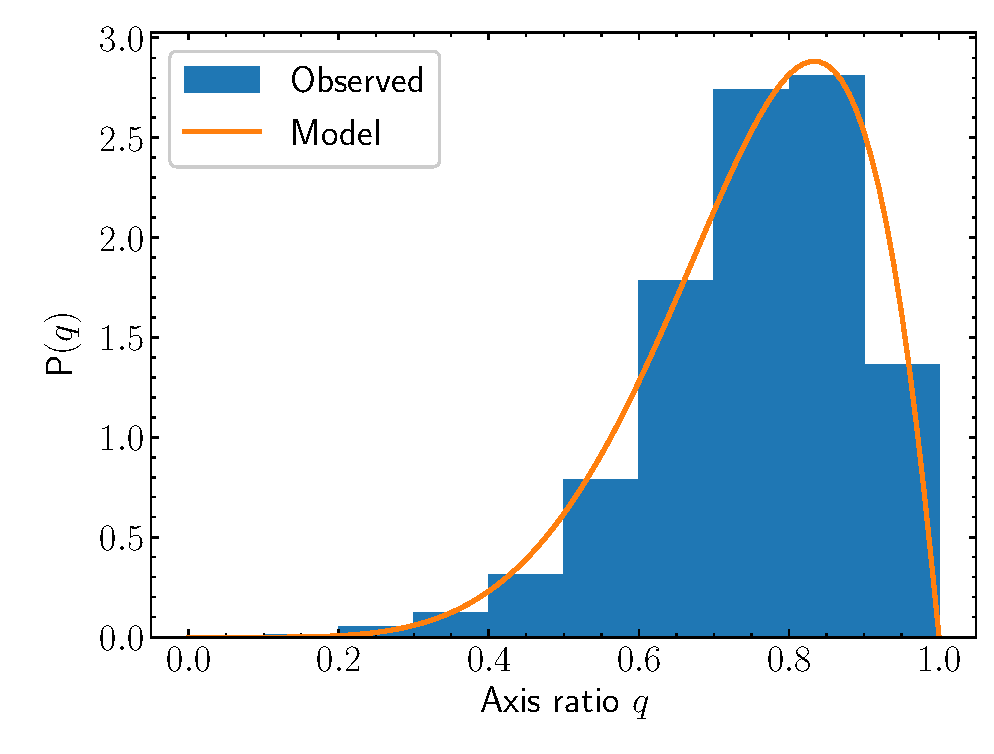
\includegraphics[width=\columnwidth]{q_dist.eps}
\caption{
Distribution in axis ratio of a sample of early-type galaxies.
The sample consists of $8078$ galaxies from the SDSS, selected by means of cuts in redshift, colour and S\'{e}rsic index as explained in the text.
Measurements of the axis ratio are taken from the de Vaucouleurs model fits of \citet{Mee++15}.
The model curve is a beta distribution, \Eref{eq:betaappendix}, with $\alpha=6.28$ and $\beta=2.05$.
}
\end{figure}

\end{document}


